% Hypergraph (vertical layout) for V={v1,v2,v3}, E={e1={v1,v2}, e2={v2,v3}}.
% Vertices are nodes; hyperedges are solid enclosing regions overlapping on v2.
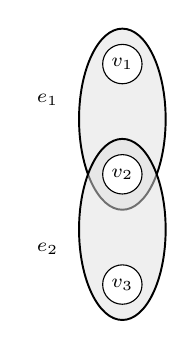
\begin{tikzpicture}[
    vertex/.style={circle, draw, fill=white, font=\scriptsize,
                   minimum size=0.5cm, inner sep=1pt},
    hedge/.style={draw, line width=0.7pt, fill=gray!25, fill opacity=0.5}
  ]

  % --- hyperedges (drawn first, behind the vertices) ---
  \draw[hedge] (0,-0.7) ellipse [x radius=0.55, y radius=1.15];
  \draw[hedge] (0,-2.1) ellipse [x radius=0.55, y radius=1.15];

  % --- hyperedge labels ---
  \node[font=\scriptsize] at (-0.95,-0.45) {$e_1$};
  \node[font=\scriptsize] at (-0.95,-2.35) {$e_2$};

  % --- vertices ---
  \node[vertex] (v1) at (0,  0  ) {$v_1$};
  \node[vertex] (v2) at (0, -1.4) {$v_2$};
  \node[vertex] (v3) at (0, -2.8) {$v_3$};

\end{tikzpicture}
